\documentclass[12pt,a4paper]{article}
\synctex=1
\usepackage[utf8]{inputenc}
\usepackage[margin=1cm]{geometry}
\usepackage{graphicx}
%\usepackage{verbatim}
\usepackage{amsmath}
\usepackage{amsfonts}
\usepackage{amssymb}
\usepackage{listings}
\usepackage{enumitem}
\usepackage{textcomp}
\usepackage{courier}
\usepackage{libertine}
\usepackage{pgfornament}
\usepackage{eso-pic}
\usepackage[hangul]{kotex}
\linespread{1.3}

\title{
	\centering
	\pgfornament[width=12cm,color=teal]{84}\\
	\vspace{1cm}
	\fontsize{50}{50} \selectfont {정보통신 수학 및 실습\\Lab assignment}\\
		\pgfornament[width=12cm,color=teal]{88}\\
	\vfill}
\author{
	\LARGE
	\begin{tabular}{rcc}
		\hline
		학번 : & 2016110056 & 2012112130\\ 
		이름 : & 박승원 & 노희승\\
		편성 : & 20조 & \today\\
		\hline
	\end{tabular}\vspace{1cm}
	\\

\includegraphics[width=0.5\textwidth]{logo.jpg}
	}
\date{}

\begin{document}
\maketitle
\pagenumbering{gobble}
\noindent
\lstset{language=matlab, columns=flexible, tabsize=4, frame=shadowbox, showstringspaces=false, breaklines=true, upquote=true, basicstyle=\normalsize}

\renewcommand{\thesubsubsection}{\alph{subsubsection})}
\renewcommand{\thesubsection}{\arabic{subsection}.}
\newpage

\section*{Chapter 4. Lab Assignment}

\subsection{Let c1=4+5j and c2=1-6j.  Answer the following questions using MATLAB.} 
\subsubsection{a = c1 - c2} 
\subsubsection{b = c1*c2}
\subsubsection{c = c1/c2} 
\subsubsection{The magnitude of c1} 
\subsubsection{The phase of c2} 
\begin{lstlisting}
>> c1 = 4 + 5i
c1 =  4 + 5i
>> c2 = 1-6j
c2 =  1 - 6i
>> a = c1 - c2
a =   3 + 11i
>> b = c1 * c2
b =  34 - 19i
>> c = c1 / c2
c = -0.70270 + 0.78378i
>> abs(c1)
ans =  6.4031
>> angle(c2)
ans = -1.4056
\end{lstlisting}

\subsection{Let $z1=3(\cos\dfrac{\pi}{3}+j\sin\dfrac{\pi}{3})\quad z2 = 5(\cos\dfrac{\pi}{4}+j\sin\dfrac{\pi}{4})$, answer the following questions:} 
\subsubsection{z1*z2.} 
\subsubsection{z2/z1}
\subsubsection{$(z1)^3+2*(z1)^2+5*z1+1$}
\begin{lstlisting}
	>> z1 = 3*(cos(pi/3) + j*sin(pi/3))
	z1 =  1.5000 + 2.5981i
	>> z2 = 5*(cos(pi/4) + j*sin(pi/4))
	z2 =  3.5355 + 3.5355i
	>> z1*z2
	ans =  -3.8823 + 14.4889i
	>> z2/z1
	ans =  1.60988 - 0.43137i
	>> z1^3+2*z1^2+5*z1+1
	ans = -27.500 + 28.579i
\end{lstlisting}
\begin{lstlisting}
>> z1 = 3*e^(i*pi/4)
z1 =  2.1213 + 2.1213i
>> z1 = 3*e^(i*pi/3)
z1 =  1.5000 + 2.5981i
>> z2 = 5*e^(I*pi/4)
z2 =  3.5355 + 3.5355i
>> z1*z2
ans =  -3.8823 + 14.4889i
>> z2/z1
ans =  1.60988 - 0.43137i
>> z1^3+2*z1^2+5*z1+1
ans = -27.500 + 28.579i
\end{lstlisting}

\subsection{Let w = 10*pi, t = [0:0.01:5].  Also let p1 = 3exp(i*(wt+pi/3)), p2 = 5*exp(i*wt+pi/4)).  Answer the following questions.} 
\subsubsection{Plot p1 using x=real(p1), y=imag(p1), z=t, and plot3(x,y,z).} 
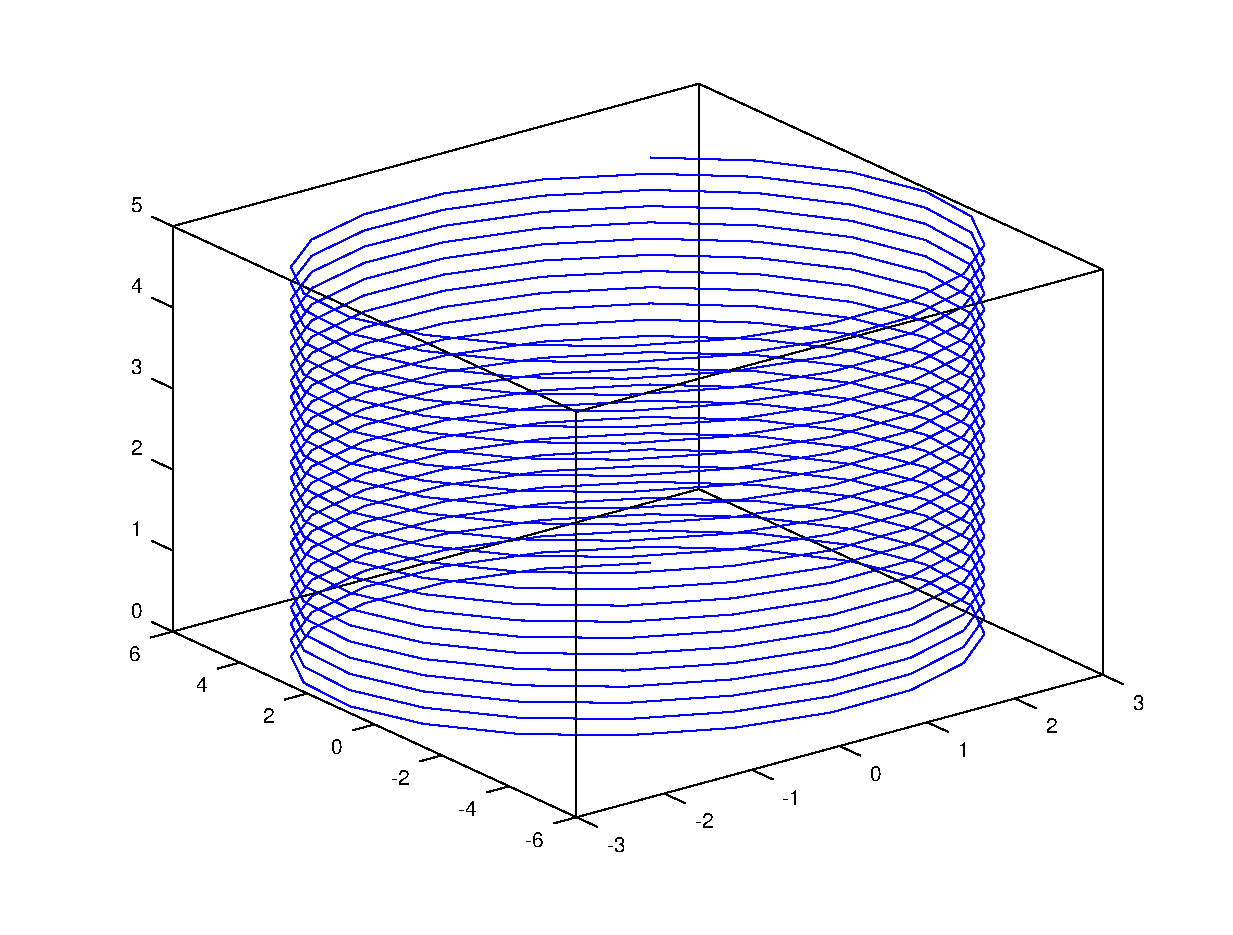
\includegraphics[width=\textwidth]{3a.eps}
\subsubsection{Find the frequency of p1 by rotating the figure drawn in (a) and see the graph on either x axis or y axis.}
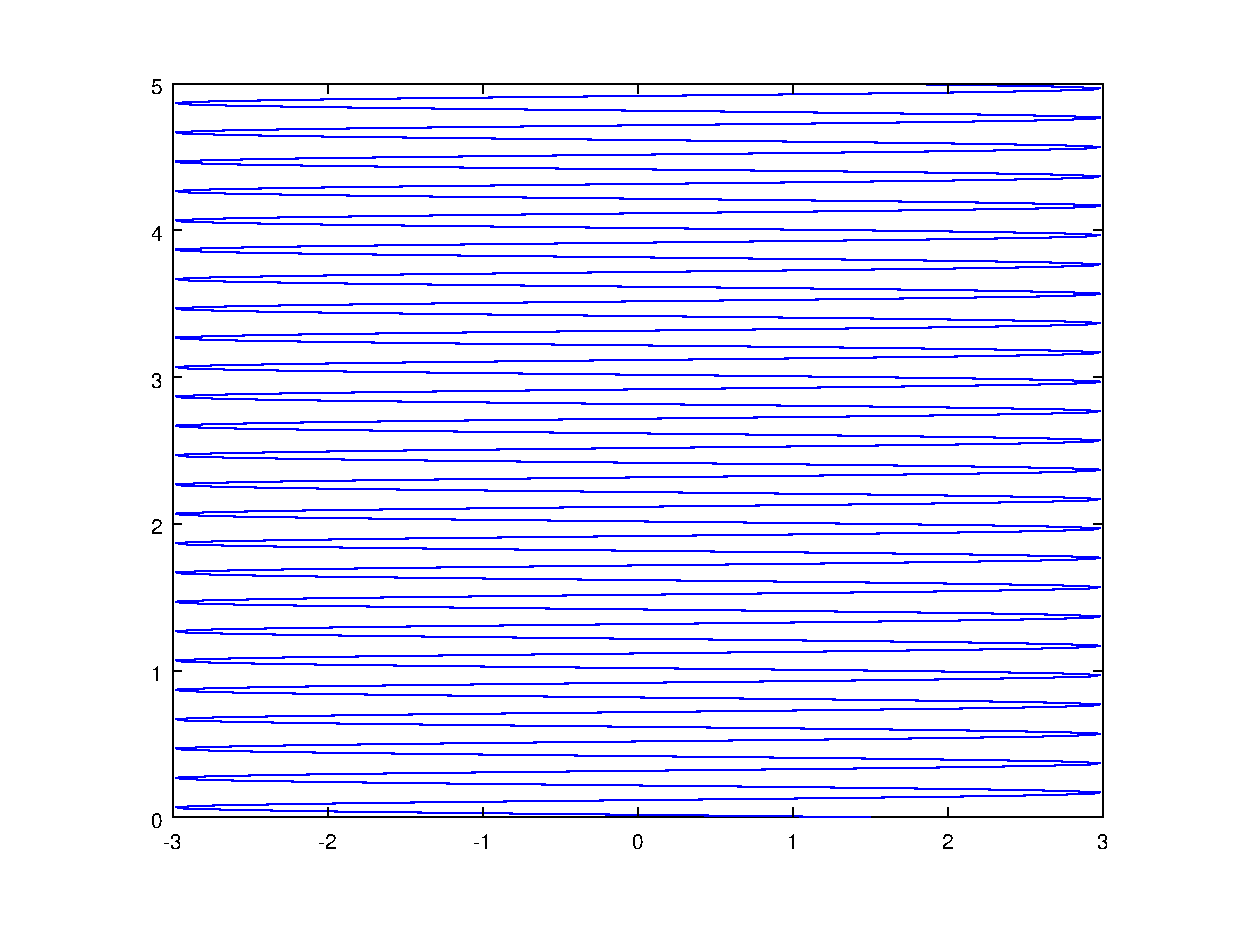
\includegraphics[width=0.8\textwidth]{3b.eps}

세로축(시간)의 1당 약 5번의 주기가 반복된다.
\subsubsection{Plot p2 using the same way as (a).  Overlay p2 on p1 using hold on command and use red ink using plot3(x, y, z, ‘r’).}
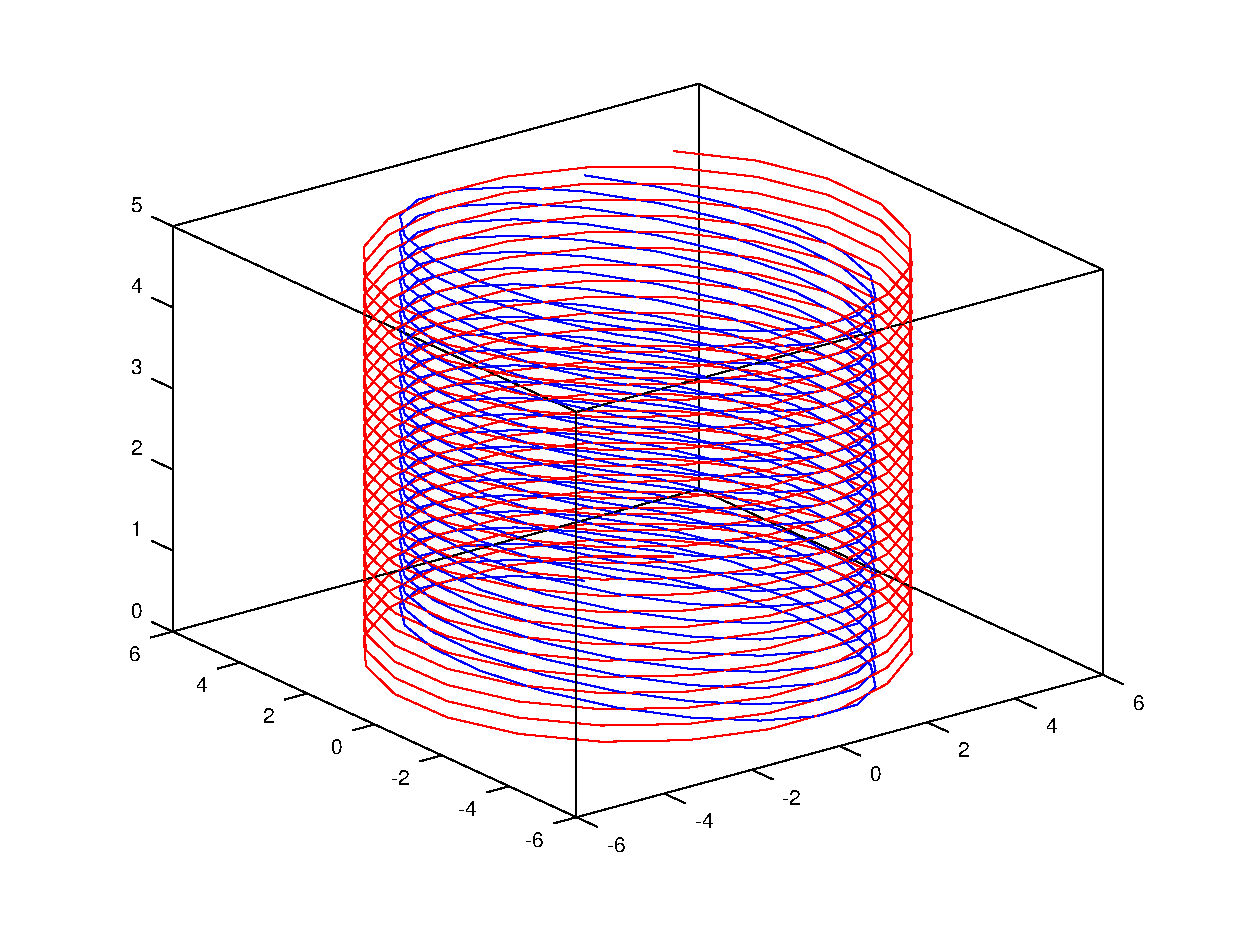
\includegraphics[width=0.8\textwidth]{3c.eps}
\subsubsection{Plot p3=p1+p2.  Overlay p1, p2, p3 on the same page using hold on command and use amber ink using plot3(x, y, z, ‘y’)..} 
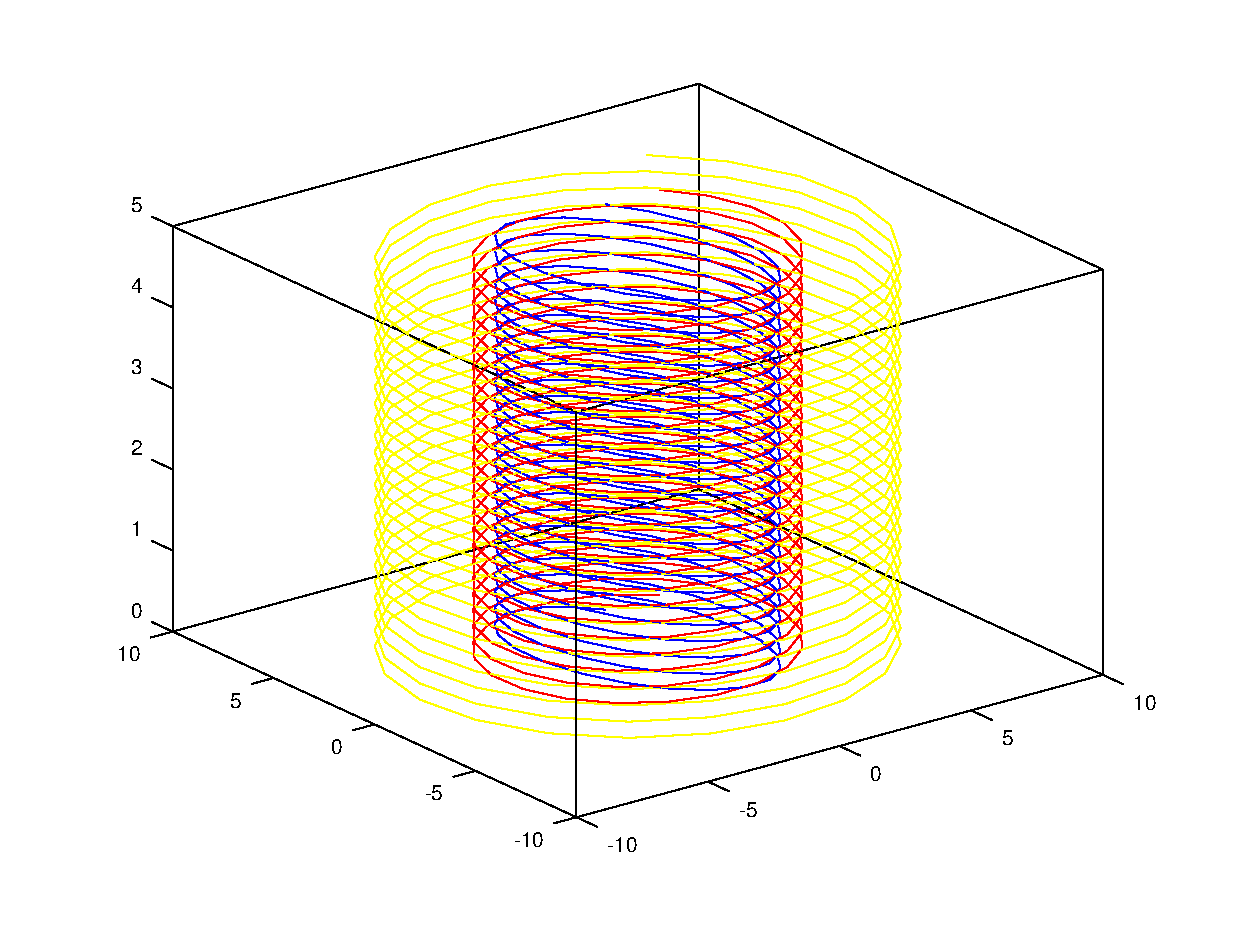
\includegraphics[width=\textwidth]{3d.eps}

\end{document}
